Dado los escasos casos de uso que se han implementado a lo largo del proyecto, no se consider'o necesario una base de datos muy sofisticada. As'i creamos una base de datos ''Hospital'', con dos tablas, una para datos del personal del hospital, ''tablaMedicos'', y otra para datos de pacientes, ''tablaPacientes''.

\begin{verbatim}
+--------------------+
| Tables_in_Hospital |
+--------------------+
| tablaMedicos       |
| tablaPacientes     |
+--------------------+
\end{verbatim}

La tabla ''tablaMedicos'' tiene dos entradas, usuario y clave, correspondientes con los datos que tienen que introducir los m'edicos cada vez que quieren iniciar sesi'on en el PDA:
\newpage
\begin{verbatim}
+---------+--------+
| USUARIO | CLAVE  |
+---------+--------+
| HOUSE   | STACY  |
| CAMERON | ISLA   |
| FOREMAN | CARCEL |
+---------+--------+
\end{verbatim}

La tabla ''tablaPacientes'' tiene tres entradas correspondientes con el nombre del paciente, la ruta en la que se encuentran almacenados en el servidor del hospital sus 'ultimos an'alisis y su expediente:

\begin{figure}[h]
	\begin{center}
		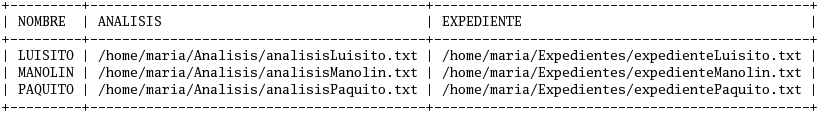
\includegraphics[scale=0.55]{bd.png}
     	\end{center}
\end{figure}

El servidor MySQL est'a continuamente funcinando en el servidor del hospital de manera que en cualquier momento son posibles los accesos a la base de datos tanto para login de los m'edicos con su PDA como para consulta de documentos de los pacientes. Estas consultas a la base de datos se hacen a trav'es de Java, gracias al paquete java.sql de J2SE.